\chapter{Special Relativity}
There are 3 fundamental effects of special relativity
\begin{itemize}
    \item Loss of simultaneity
    \item Time dilation
    \item Length contraction
\end{itemize}
\section{kinematics}
Let the frame $S'$ be moving at speed $v$ relative to a stationary frame $S$. Denote all quantities (for e.g. time) in the $S'$ frame with a prime ($'$).  
\subsection{basics}
\textbf{Time dilation}
\begin{equation}
    t'=\frac{t}{\gamma}=\gamma t'
\end{equation}
\textbf{Length contraction}
\begin{equation}
    \ell'=\gamma\ell = \frac{\ell'}{\gamma}
\end{equation}
where $\gamma=1/\sqrt{1-\frac{v^2}{c^2}}$
Since $c$ is the maximum possible speed a thing can reach, $\gamma$ will always be \textbf{greater than or equal to} 1. 
\subsection{Lorentz transformation}
\begin{equation}
    \begin{cases}
      \Delta x= \gamma (\Delta x' + v \Delta t') \\
      \Delta t= \gamma (\Delta t'+v \frac{\Delta x'}{c^2})\\
    \end{cases}      
\end{equation} 
or
\begin{equation}
    \begin{cases}
      \Delta x'= \gamma (\Delta x - v \Delta t) \\
      \Delta t'= \gamma (\Delta t - v \frac{\Delta x}{c^2})\\
    \end{cases}      
\end{equation} 

To derive the equation for time dilation, we note that the person measuring it (either in $S$ or $S'$) has to be stationary (i.e. $v=0$).

From the equation above and setting $\Delta x'$ to 0, we see that $\Delta t=\gamma \Delta t'$. Since $\gamma\geq 1$, the time elapsed measured by the stationary observer in the $S'$ frame is always shorter than the time elapsed in $S$. 

However, if we set $\Delta x$ to 0 and use the second set of equation, we get $\Delta t'=\gamma \Delta t$. This seems to be a contradiction. But in fact, this scenario is very different as the stationary observer is now in the $S$ frame (and not the $S'$ frame).

\subsection{relativistic velocity addition}
Let $v_1$ be the speed of the object measured in the frame: $S'$ moving at speed $v_2$ relative to the ground.

Writing out the lorentz transformation for $S'$, we get 

\begin{equation}
    \begin{cases}
        \Delta x= \gamma_2 (\Delta x'+v_2 \Delta t')\\
        \Delta t = \gamma_2 (\Delta t'+v_2 \frac{\Delta x'}{c^2})\\
    \end{cases}
\end{equation}
where $\gamma_2$ is the Lorentz factor associated with $v_2$.
As the speed measured in the lab frame ($S$) is defined as $\Delta x/\Delta t$, we get 
\begin{equation}
    \frac{\Delta x}{\Delta t}= \frac{\gamma_2 (\Delta x'+v_2 \Delta t')}{\gamma_2 (\Delta t'+v_2 \frac{\Delta x'}{c^2})} = \frac{v_1+v_2}{1+(v_1 v_2)/c^2}
\end{equation}
The derivation \textbf{above} only applies to velocity addition in the \textbf{longitudinal direction}. For \textbf{transverse velcoity addition}, we can use a similar method (Lorentz transformation: $\Delta y'=\Delta y= v \Delta t $)
\begin{equation}
    \frac{\Delta y}{\Delta t}=\frac{\Delta y'}{\gamma (\Delta t'+v \frac{\Delta x'}{c^2})} =\frac{\Delta y'/\Delta t'}{\gamma (1 +v \frac{\Delta x'/\Delta t'}{c^2})}= \frac{v_y'}{\gamma (1+v'_x\frac{v}{c^2})}
\end{equation}
I think this could be easily derived using 4-vectors, but becuase i havent learnt that yet, so idk LMAO. 

\subsection{invariance and minkowski diagram}
Consider the quantity $(\Delta s)^2= c^2(\Delta t)^2- (\Delta x)^2$, where $s$ (dropping the $\Delta$ from now on) is known as the \textbf{invariant interval} because this quantity is invariant to coordinates (i.e. $ct-x=ct'-x'$, $(ct, x)$ is usually known as the \textbf{spacetime interval}). 

\begin{figure}[H]
    \centering
    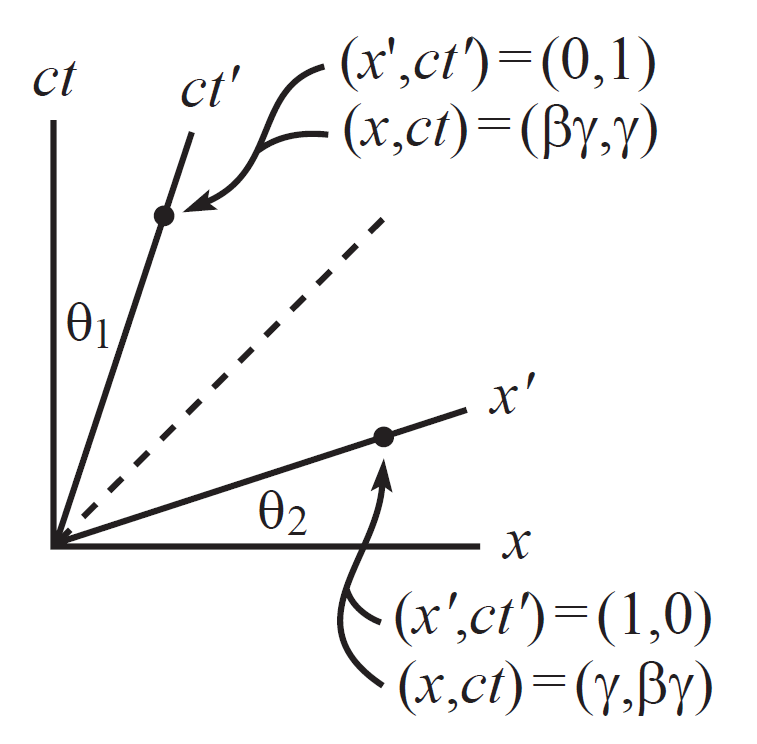
\includegraphics[width=0.3\textwidth]{minkowski.png}
\end{figure}
This could be derived with \textbf{lorentz transformation} with $\beta =v/c$. 1 unit on the $ct$ axis would correspond to $\gamma\sqrt{(1+\beta^2)}$ on the $ct'$ axis. Hence,
\begin{equation}
    \frac{\textsf{one} \ ct' \ \textsf{unit}}{\textsf{one} \ ct \ \textsf{unit}}=\frac{\sqrt{1+\beta^2}}{\sqrt{1-\beta^2}}
\end{equation}

Simultaenous measurements can be represented by drawing a line perpendicular to the $ct$/$ct'$ axes and seeing the points of intersection of the line with the $ct$/$ct'$ axes. 

\section{dynamics}
\subsection{Energy and momentum}
\textbf{Energy}
\begin{equation}
    E=\gamma m c^2
\end{equation}
\textbf{Momentum}
\begin{equation}
    \mathbf{p}=\gamma m \mathbf{v}
\end{equation}
To justify these expressions, I think it is quite elegant to perform Taylor series expansion in the limit of $v \ll c$ for $1/\sqrt{1-x^2}$ \footnote{$(1+x)^{-\frac{1}{2}}=1-\frac{1}{2}x+\frac{3}{8}x^2-\frac{5}{16}x^3+\frac{35}{128}x^4...$}, you obtain

\begin{equation}
    \begin{cases}
        E=mc^2(1+\frac{1}{2}(\frac{v}{c})^2+\frac{3}{8}(\frac{v}{c})^3+\frac{5}{16}(\frac{v}{c})^4+...)=mc^2+\frac{1}{2}mv^2+...\\
        \mathbf{p}=m \mathbf{v}(1+\frac{1}{2}(\frac{v}{c})^2+\frac{3}{8}(\frac{v}{c})^3+\frac{5}{16}(\frac{v}{c})^4+...)=m\mathbf{v}+...\\
    \end{cases}
\end{equation}

There is this very important equation
\begin{equation}
    E^2=p^2c^2+m^2c^4
\end{equation}
Another pretty useful equation is from the fundamental equations describing relativistic momentum and energy, 
\begin{equation}
    \frac{\mathbf{p}}{E}=\frac{\mathbf{v}}{c^2}
\end{equation}

Moreover, the equations to convert energy and momentum between frames are also quite elegant. Let the particle be travelling at speed $v$ in frame $S'$, which is moving at speed $u$ relative to lab frame $S$, then the energy and momentum in the 2 frames are related through
\begin{equation}
    \begin{cases}
        E=\gamma_u(E'+vp')\\
        p=\gamma_u(p'+vE')\\
    \end{cases}
\end{equation} \footnote{$E'=\gamma_v m$ and $p'=\gamma_v m v$, note that it is $\gamma_v$ and not $\gamma_u$}

Through this equation, we note that $E$ and $p$ behave exactly the same way as $ct$ and $x$. Hence, we obtain the following equation
\begin{equation}
    m^2=E^2-p^2=E'^2-p'^2
\end{equation}
where the mass of the particle, $m$, is the \textbf{invariant quantity}.

\subsection{Relativistic Collisions}
It is important to note that this $E=\gamma mc^2$ here is not equivalent to kinetic energy($E-mc^2$). During collision, it is the \textbf{total energy} that is conserved, so always use $E$ and not KE. 

To solve collisions problems, it is nice to define a \textbf{4- momentum}, or $P=(E,p_x,p_y,p_z)$ \footnote{Note that it shld be $E/c$ to make it dimensionally consistent but since $c=1$, we can just write it like this}. The inner product of this "vector" is defined to be $a_1b_1-a_2b_2-a_3b_3-a_4b_4$. It is defined this way so that we can concisely write $m^2=E^2-p^2$ as 
\begin{equation}
    P\cdot P=m^2
\end{equation}

\subsection{Force}






\section{4-vector}
The most basic 4-vector is the \textbf{4-displacement} between two points in spacetime, which we call events. The 4-displacement is a fundamentally invariant geoemtric object, which you can think of as an arrow pointing between these 2 events. 

Consider two inertial frame $S$ and $S'$, such that $S'$ is moving at speed $v$ in the positive x-direction relative to $S$. Their coordinates are calibrated such that their origins coincide at $t=t'=0$. The frames are said to be in \textbf{standard configuration}, and their change-of-coordinates transformation can be summarised by the following
\begin{equation}
    \begin{bmatrix}
        ct' \\
        x' \\ 
        y' \\ 
        z'
    \end{bmatrix}
    =
    \begin{bmatrix}
        \gamma & \beta \gamma &  & \\
        -\beta \gamma & \gamma &  & \\ 
         &  & 1 & \\ 
         &  &  & 1
    \end{bmatrix}
    \begin{bmatrix}
        ct\\
        x \\ 
        y \\ 
        z
    \end{bmatrix}
\end{equation}
This is lorentz transformation in the matrix form, where the transformation matrix is known as the \textbf{lorentz boost} to boost from the $S$ frame to the $S'$ frame.


